%%%%%%%%%%%%%%%%%%%%%%%%%%%%%%%%%%%%%%%%%
% a0poster Landscape Poster
% LaTeX Template
% Version 1.0 (22/06/13)
%
% The a0poster class was created by:
% Gerlinde Kettl and Matthias Weiser (tex@kettl.de)
% 
% This template has been downloaded from:
% http://www.LaTeXTemplates.com
%
% License:
% CC BY-NC-SA 3.0 (http://creativecommons.org/licenses/by-nc-sa/3.0/)
%
%%%%%%%%%%%%%%%%%%%%%%%%%%%%%%%%%%%%%%%%%

%----------------------------------------------------------------------------------------
%	PACKAGES AND OTHER DOCUMENT CONFIGURATIONS
%----------------------------------------------------------------------------------------

\documentclass[a0,landscape]{a0poster}

\usepackage{multicol} % This is so we can have multiple columns of text side-by-side
\columnsep=90pt % This is the amount of white space between the columns in the poster
\columnseprule=3pt % This is the thickness of the black line between the columns in the poster

\usepackage[svgnames]{xcolor} % Specify colors by their 'svgnames', for a full list of all colors available see here: http://www.latextemplates.com/svgnames-colors

\usepackage{times} % Use the times font
%\usepackage{palatino} % Uncomment to use the Palatino font
\usepackage{float} % Allows putting an [H] in \begin{figure} to specify the exact location of the figure
\usepackage{graphicx} % Required for including images
\graphicspath{{figures/}} % Location of the graphics files
\usepackage{booktabs} % Top and bottom rules for table
\usepackage[font=small,labelfont=bf]{caption} % Required for specifying captions to tables and figures
\usepackage{amsfonts, amsmath, amsthm, amssymb} % For math fonts, symbols and environments
\usepackage{wrapfig} % Allows wrapping text around tables and figures
\usepackage[center]{titlesec}
\usepackage{background}
\usepackage{blindtext}
\usepackage{euler}
\backgroundsetup{
scale=1,
angle=0,
opacity=1,
contents={\begin{tikzpicture}[remember picture,overlay] 
\path [bottom color = Maroon!20!white, top color = white] (current page.south west)rectangle (current page.north east);\end{tikzpicture}}
}
\begin{document}

%----------------------------------------------------------------------------------------
%	POSTER HEADER 
%----------------------------------------------------------------------------------------

% The header is divided into three boxes:
% The first is 55% wide and houses the title, subtitle, names and university/organization
% The second is 25% wide and houses contact information
% The third is 19% wide and houses a logo for your university/organization or a photo of you
% The widths of these boxes can be easily edited to accommodate your content as you see fit

\begin{minipage}[b]{0.5\textwidth}
\veryHuge \color{Brown} \textbf{Radio Cosmology Lab} \color{Black}\textbf{$|$} \color{Black}\LARGE\textit{Exploring the Epoch of Reionization}\\
\textbf{Adam Lanman, Wenyang Li, Joshua Kerrigan, Jacob Burba, \\Peter Sims, Daniya Seitova, Jonathan Pober}\\ % Author(s)
\huge Brown University Physics\\ % University/organization
\end{minipage}
\begin{minipage}[b]{0.6\linewidth}

\includegraphics[width=45cm]{radiologo_update.png} % Logo or a photo of you, adjust its dimensions here
\end{minipage}
%I CANT SEEM TO GET THIS DAMN LOGO TO THE RIGHT

%[Maybe put logos at the top(or bottom), PAPER doesn't have an official logo afaik, can't find a good one for MWA]
%\hspace{5cm}
%\begin{minipage}[b]{0.15\linewidth}
%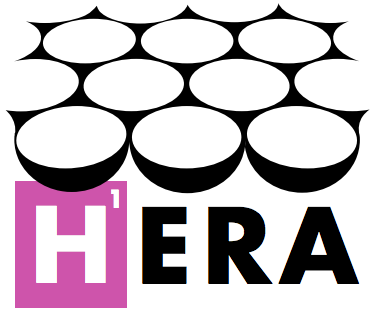
\includegraphics[width=15cm]{HERA.png} % Logo or a photo of you, adjust its dimensions here
%\end{minipage}
%\hspace{2cm}
%\begin{minipage}[b]{0.15\linewidth}
%\Huge{\textbf{PAPER}}
%\end{minipage}
%\hspace{2cm}
%\begin{minipage}[b]{0.15\linewidth}
%\Huge{\textbf{MWA}}
%\end{minipage}

%
%\begin{minipage}[b]{0.25\linewidth}
%\color{DarkSlateGray}\Large \textbf{Contact Information:}\\
%Physics\\ % Address
%Brown University\\
%$\#$ George St., Providence, RI\\\\
%Phone: +1 (000) 111 1111\\ % Phone number
%Email: \texttt{Add Emails}\\ % Email address
%\end{minipage}
%
% Maybe we don't need the Brown logo, consider replacing with PAPER,HERA,MWA logos?


%\vspace{1cm} % A bit of extra whitespace between the header and poster content

%----------------------------------------------------------------------------------------

\begin{multicols}{4} % This is how many columns your poster will be broken into, a poster with many figures may benefit from less columns whereas a text-heavy poster benefits from more

%----------------------------------------------------------------------------------------
%	ABSTRACT
%----------------------------------------------------------------------------------------

%\color{Navy} % Navy color for the abstract

%\begin{abstract}

%Following the recombination of hydrogen and release of the cosmic microwave background radiation at redshift $z \sim 1100$, the baryonic matter of the universe consisted mostly of neutral hydrogen and helium. Gradually, small inhomogeneities collapsed and ignited the first luminous structures. Energetic photons emitted from the first stars and quasars reionized the surrounding medium, producing ionized bubbles which grew and merged into the fully ionized intergalactic medium we see today. This \emph{Epoch of Reionization} (EoR) remains a poorly-understood period of the universe's history which offers a wealth of cosmological and astrophysical information.

%The Pober lab is part of an international effort to build instruments capable of studying the EoR. The neutral hydrogen (HI) of the EoR emits faintly at a wavelength of 21cm, due to the hyperfine transition. This emission is unique to neutral hydrogen, and is anti-correlated with the ionized (HII) regions that fill the universe through the EoR. CMB constraints and quasar absorption spectra put the EoR as occurring within the redshift range $6 < z < 12$, which means 21cm emissions will redshift to meter scale wavelengths. This is accessible to modern radio interferometers, including the \emph{Donald C. Backer Precision Array for Probing the Epoch of Reionization} (PAPER), the \emph{Murchison Widefield Array} (MWA), and the recently-funded \emph{Hydrogen Epoch of Reionization Array} (HERA).

%The main focus of the Pober Lab is the direct observation of the 21cm Neutral Hydrogen (HI) emission through the use of radio telescope arrays to detect the signal from the Epoch of Reionization (EoR). The 21cm hyperfine spin flip, which is typically a forbidden transition, has a mean lifetime on the order of 100 million years. This time scale, and the abundance of HI in the universe gives us the ability to map the progress of reionization which has the redshift range of 6 $<$ z $<$ 12. To observe the reionization of the HI, we use radio telescope arrays, because the 21cm emission corresponds to 1420 MHz at rest and when received at Earth corresponds to 100-200 MHz due to cosmological redshifting. The Pober Lab contributes to several international radio telescope array collaborations which include the Precision Array for Probing the Epoch of Reionization (PAPER), the Murchison Widefield Array (MWA) and the newly NSF funded Hydrogen Epoch of Reionization Array (HERA).

%\end{abstract}

%----------------------------------------------------------------------------------------
%	INTRODUCTION
%----------------------------------------------------------------------------------------
\color{DarkSlateGray}  % SaddleBrown color for the introduction

\section*{Introduction}
Following the recombination of hydrogen and release of the cosmic microwave background radiation, the baryonic matter of the universe consisted mostly of neutral hydrogen and helium. Gradually, small inhomogeneities collapsed and ignited into the first luminous structures. Energetic photons emitted from the first stars and quasars reionized the surrounding medium, producing ionized bubbles which grew and merged into the fully ionized intergalactic medium we see today. This \emph{Epoch of Reionization} (EoR) remains a poorly-understood period of the universe's history which offers a wealth of cosmological and astrophysical information.

The Pober lab is part of an international effort to build instruments capable of studying the EoR. The neutral hydrogen (HI) of the EoR emits faintly at a wavelength of 21cm due to the hyperfine transition. This emission is unique to neutral hydrogen, and is anti-correlated with the ionized (HII) regions that fill the universe through the EoR. CMB constraints and quasar absorption spectra place the EoR within the redshift range $6 < z < 12$, which means 21cm emissions will reach us at meter scale wavelengths. This is accessible to modern radio interferometers, including the \emph{Donald C. Backer Precision Array for Probing the Epoch of Reionization} (PAPER), the \emph{Murchison Widefield Array} (MWA), and our newly observing \emph{Hydrogen Epoch of Reionization Array} (HERA). Extracting this weak signal remains a challenge unprecedented in radio astronomy.



\subsubsection*{Differential Brightness Temperature}
%\begin{equation}
%\label{difftemp}
%\resizebox{.9\hsize}{!}{$
%\delta T_{b} = 28mK(1+\delta)x_{HI}\Big(1-\frac{T_{CMB}}{T_{spin}}\Big)\Big(\frac{\Omega_{b}h^2}{0.0223}\Big)%\sqrt{\Big(\frac{1+z}{10}\Big)\Big(\frac{0.24}{\Omega_m}\Big)}\Big[ \frac{H(z)/(1+z)}{dv_{||}/dr_{||}}\Big]$}%
%\end{equation}

\begin{figure}[H]
\centering
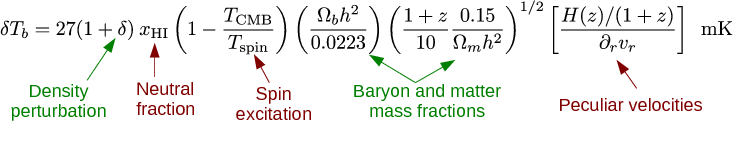
\includegraphics[scale=1]{figures/differential_brightness.png}
\end{figure}

The differential brightness temperature $\delta T_b$ is the contrast between the intensity of 21 cm emissions/absorptions against the Cosmic Microwave Background. Its full expression is related to cosmological (green) and astrophysical (red) parameters. Figure \ref{global} shows the evolution of the spherically-averaged \emph{global} 21 cm brightness temperature.

\begin{figure}[H]
\centering
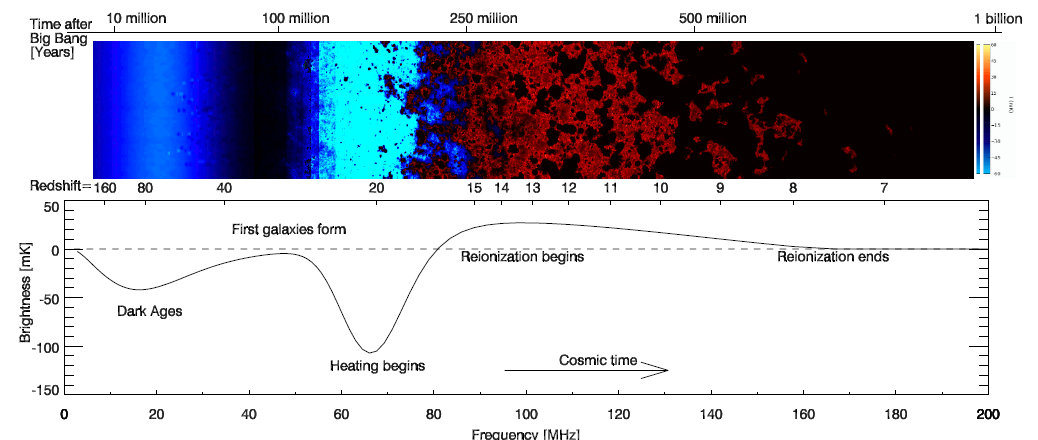
\includegraphics[width=1.0\linewidth]{figures/global_history.png}
\caption{The global differential brightness temperature, $\delta T_b$, evolution over redshift $6<z<160$. $\delta T_b$ becomes observable when the spin temperature $T_S$ decouples from the CMB temperature, $T_{CMB}$. Source: Pritchard \& Loeb. Nature 468.7325 (2010): 772-773. }\label{global}
\end{figure}

%----------------------------------------------------------------------------------------
%	OBJECTIVES
%----------------------------------------------------------------------------------------
% DarkSlateGray color for the rest of the content
%\section*{The Foreground Problem} %[I dont need all of these plots, they're just there to be cut as needed or if necessary to take up more space]
%Galactic and extragalactic foregrounds pose a difficult problem when trying to measure the 21cm EoR signal. Relative to galactic foregrounds, the EoR signal is $\sim$ 5 orders of magnitude smaller than the galactic emissions that exist between our observing radio telescope arrays and the highly redshifted 21cm signal. The overlapping sources of power in our observations can be seen in Fig. \ref{fig:foregroundsrcs}.  -- Just making this shorter, and clarifying a bit on what the foregrounds are.

The major challenge of EoR detection is the overwhelmingly bright foreground contamination. The expected EoR signal is $\sim$ 5 orders of magnitude weaker than known foreground sources, such as diffuse emission from the Galaxy and extragalactic point sources. Removing these foregrounds, as well as instrumental noise, is a nontrivial problem. In addition to galactic and extragalactic foregrounds we must also contend with Radio Frequency Interference (RFI).


%\begin{figure}[H]
%\centering
%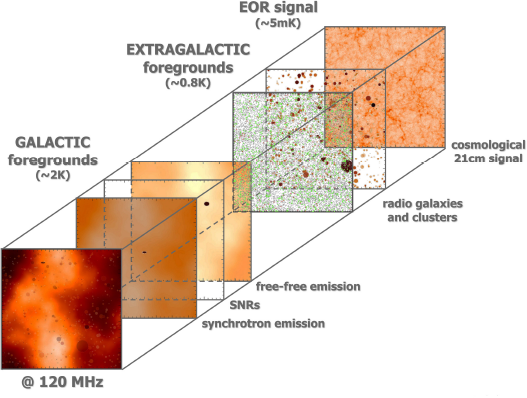
\includegraphics[width=0.55\linewidth]{figures/foreground_figure.png}
%\caption{The various cosmological and galactic sources that contribute to the measured sky temperature, and their relative strengths.\\\hspace{\textwidth}
%Source: Zaroubi, Saleem. \textit`{The First Galaxies}. Springer Berlin Heidelberg, 2013. 45-101.}\label{fig:foregroundsrcs}
%\end{figure}



\subsection*{Bayesian Data Analysis}

\vspace{-1.0cm}
\begin{figure}[H]
\begin{centering}
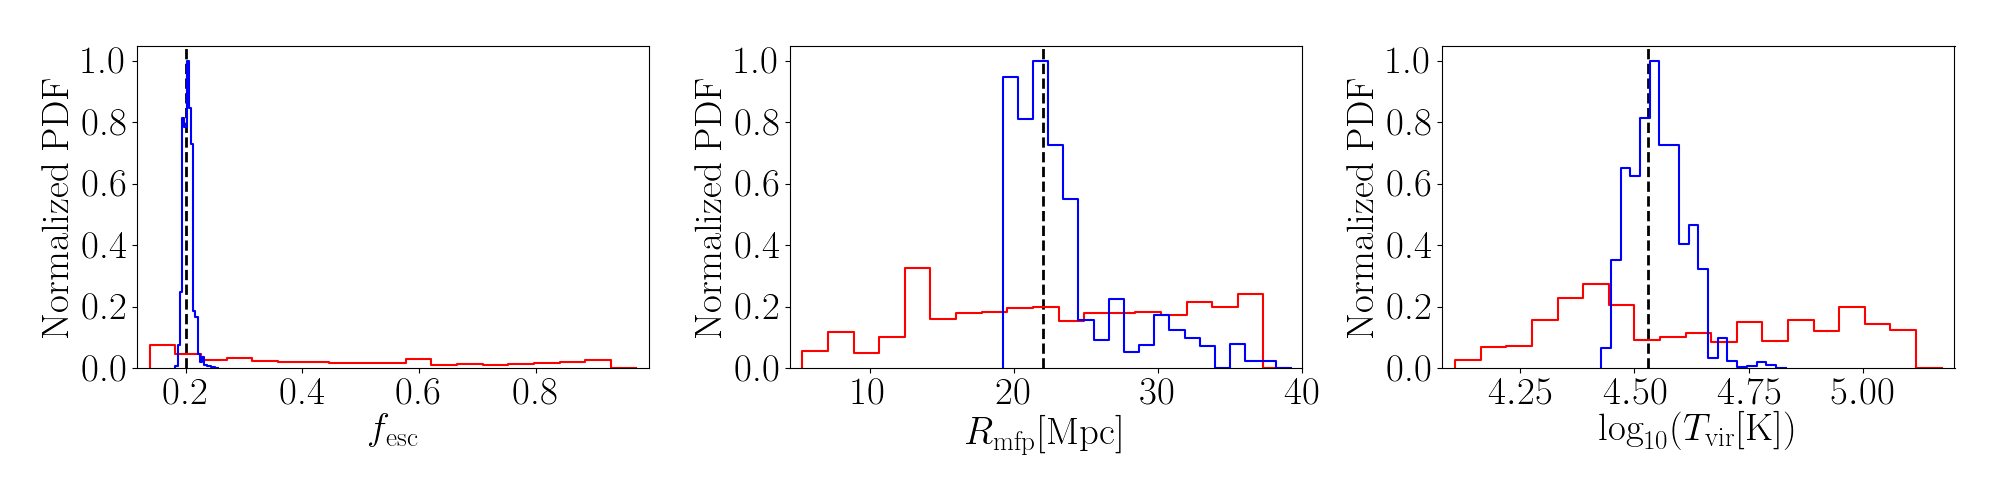
\includegraphics[width=0.9\linewidth]{Astro_constraints_lowk_comparison_3.png}\\
\vspace{-0.3cm}
{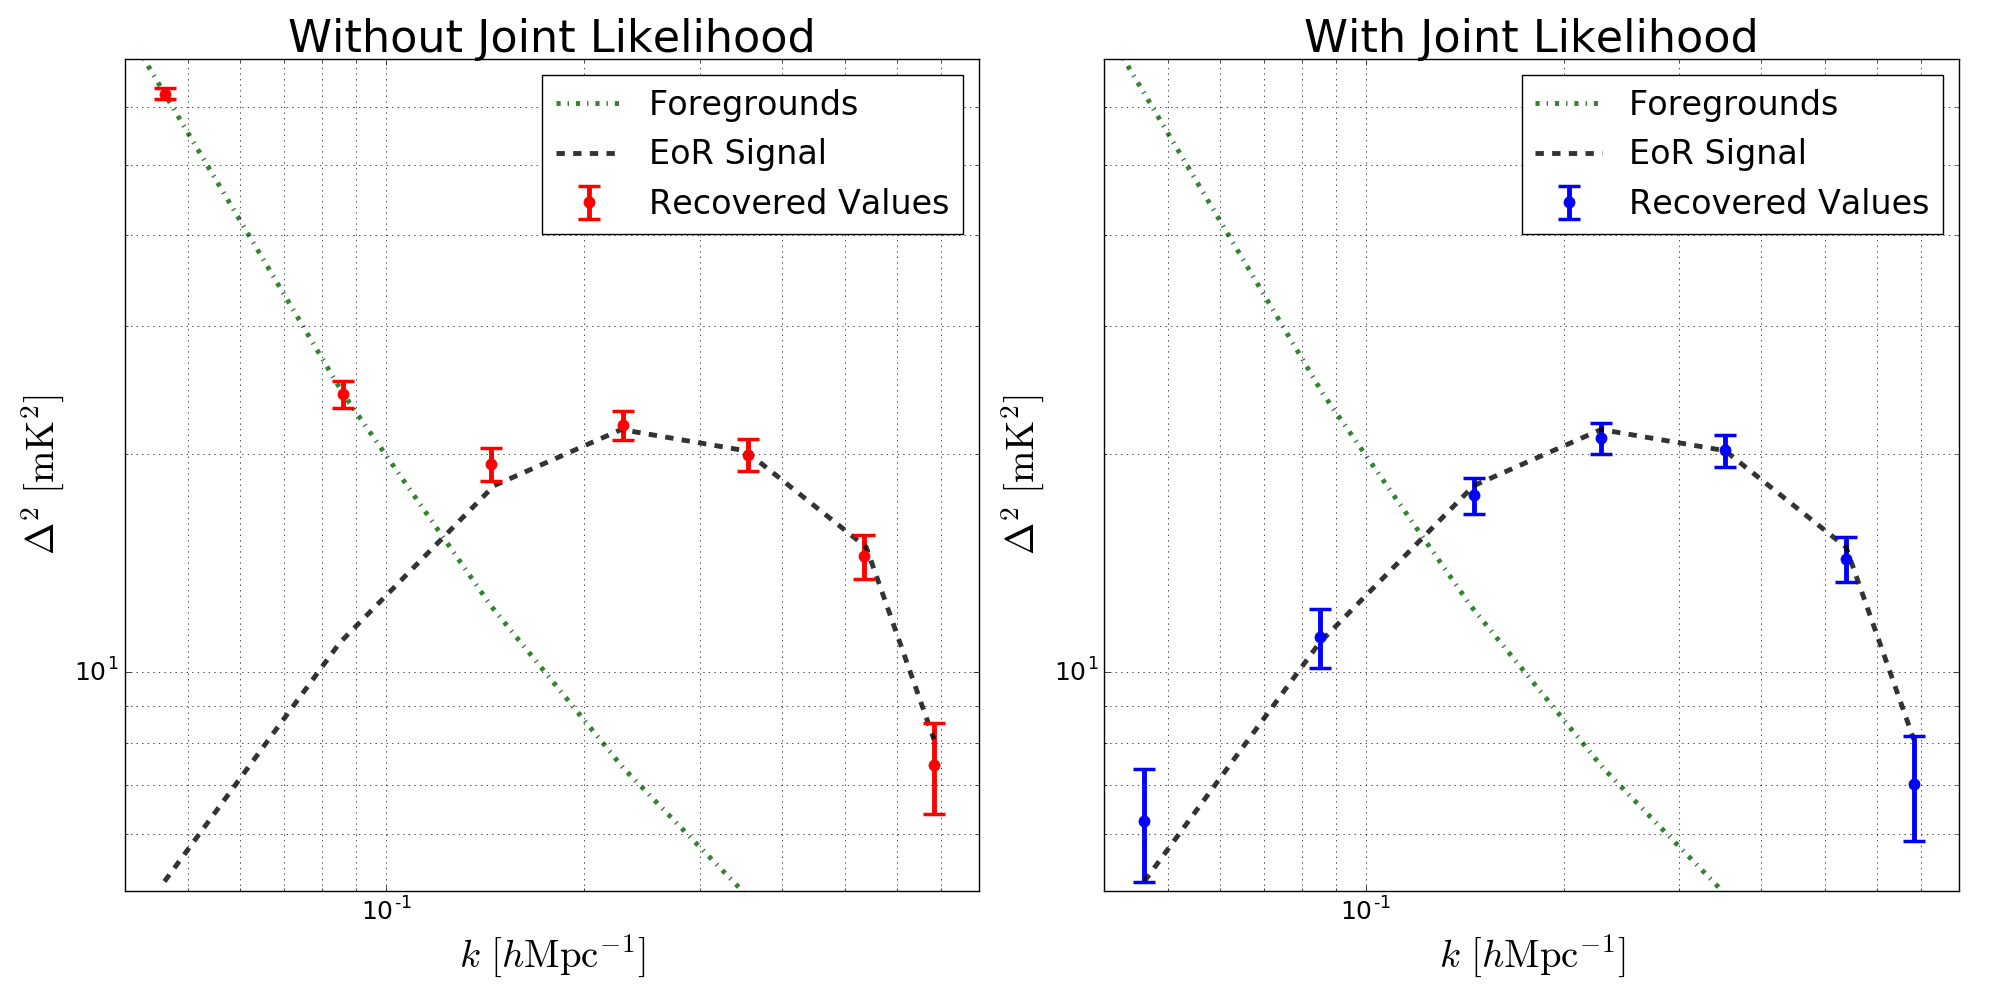
\includegraphics[width=0.9\linewidth]{JF_twopanel.png}}
\vspace{-0.1cm}
\caption{[Top] Constraints on the escape fraction of ionizing radiation from galaxies, $f_\mathrm{esc}$, the mean free path of ionizing photons through the intergalactic medium, $R_\mathrm{mfp}$, and the minimum virial temperature of halos hosting galaxies, $T_\mathrm{vir}$ derived from power spectrum estimates accessible using the existing HERA analysis pipeline (red) and Bayesian forward modeling analysis of simulated HERA data (blue). [Bottom] Recovered EoR power spectrum from simulated HERA data using a Bayesian power spectral estimation methodology with i) polynomial foreground parametrization (red points, left) and ii) an optimized power law parametrization derived using Bayesian model selection (blue points, right).}
\label{SphericalPSofEoRplusFgs_with_CylindricalFgPrior}
\end{centering}
\end{figure}

A statistically robust analysis of the data is essential to avoid a spurious or mischaracterised detection of the EoR signal. We have developed an advanced Bayesian mathematical data analysis framework designed to meet this need. By extending the range of spatial scales on which the EoR signal can be reliably measured, this framework brings forward a first detection of the EoR signal and facilitates further analysis of the data to probe the state of dark matter in the early Universe.





\subsection*{Deep Learning for RFI Mitigation}
RFI is present in all radio observations and consists of both terrestrial (e.g. TV stations) and in orbit (e.g. satellites) sources.
% This interference reduces sensitivity in 21cm EoR experiments because it can be present in nearly all frequency channels and is brighter than galactic foregrounds. 
Due to the nature of how RFI manifests itself in visibility data as sharp discontinuities or disruptive amorphous shapes, novel machine learning techniques can be applied. We introduce a Deep Fully Convolutional Neural Network 
% (D-FCN) which uses the time-frequency context from both amplitude and phase 
to form a robust and efficient method for identifying RFI.
\begin{figure}[H]
\centering
\frame{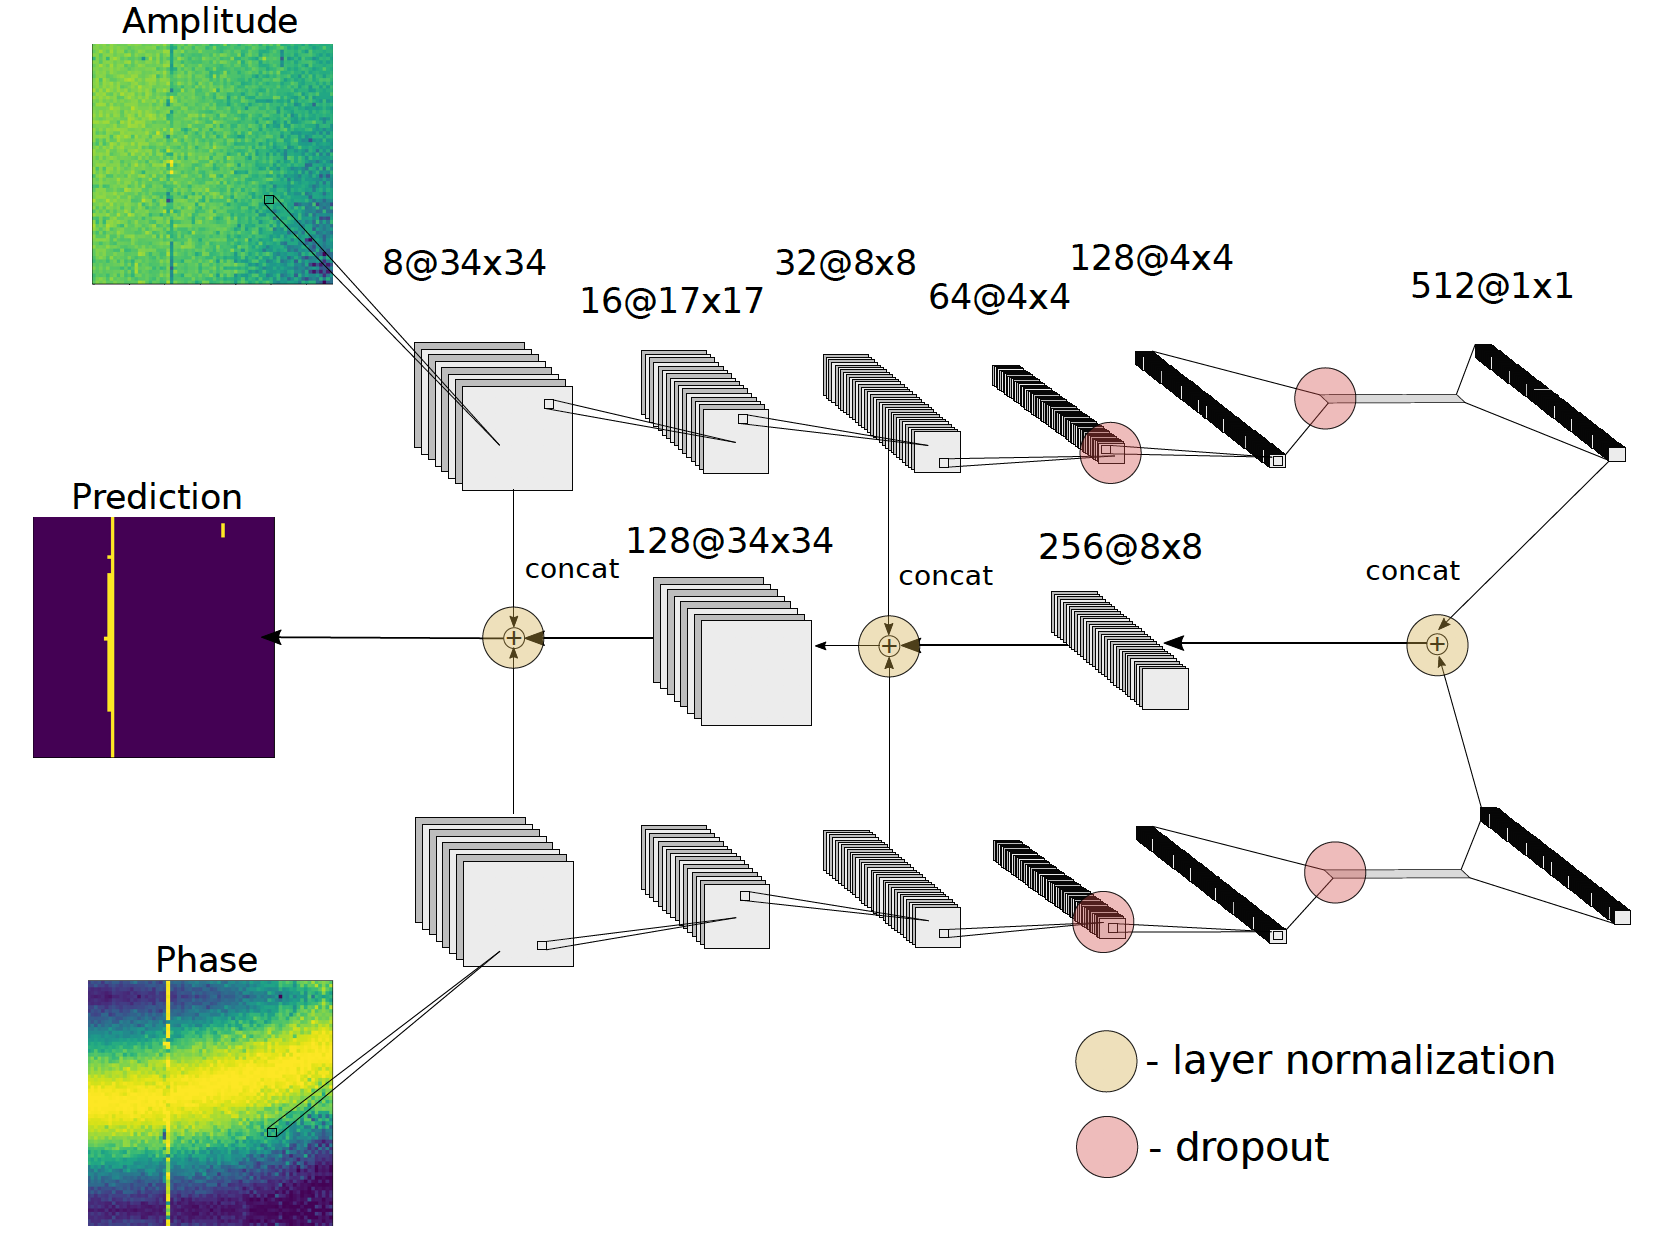
\includegraphics[width=0.8\linewidth]{figures/PostFCStitchArch_v6_1.png}}
\caption{Deep Full Convolutional Neural Network (D-FCN) architecture design for application to interferometric visibilities. The input space consists of a normalized log amplitude (upper branch) and it's corresponding phase component. Both input layers reintroduce coarse time-frequency information into the transpose convolutional layers in what's referred to as `skip connections'.}
\label{fig:DFCNArch}
\end{figure}



%----------------------------------------------------------------------------------------
%	MATERIALS AND METHODS
%----------------------------------------------------------------------------------------
\columnbreak
\section*{Simulation}

The particular characteristics of an array can introduce unexpected effects into the data. Understanding and mitigating instrumental effects is critical to making a confident detection of the EoR. For this reason, much effort has been put into simulating the full analysis pipeline -- from the point and diffuse sources on the sky, to the raw visibilities that come out of the correlator, to the power spectrum estimations.

Fast Holographic Deconvolution (FHD) is a purpose-built software framework for analyzing MWA data. FHD does foreground subtraction by \emph{forward modeling}, which builds a simulated data set, including instrumental effects, and subtracts it from the actual data. This forward modeling feature can also be used as a standalone simulation tool, to generate raw visibilities of foregrounds, noise, and EoR off of existing and future 21cm experiments.

\begin{figure}[H]
\centering
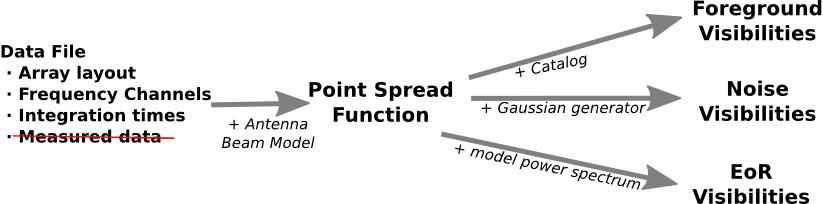
\includegraphics[scale=.9]{figures/sim_flowchart.png}
\caption{A sample data file (or generated data file) holds array coordinates over time and the frequency channels of the instrument. Given a beam model for the antenna, FHD calculates the full synthesized beam (or point-spread function) for a particular time and set of frequencies. The synthesized beam can then convert a sky catalog into a set of foreground visibilities for the instrument. External EoR simulations can also be fed in to test EoR sensitivity, or Gaussian noise can be injected to simulate noise.}
\end{figure}

%------------------------------------------------
\section*{Calibration}

%The most common techniques we use on visibility calibration are redundant calibration and sky model based calibration. Sky model calibration requires some preknowledge about the sky. With our assumptions about source structures of the sky and understanding of our instrument, we use FHD (Fast Holographic Deconvolution) to calibrate visibility data. The algorithm FHD uses is basically 'CLEAN' algorithm. Redundant calibration is sky model independent. All it assumes is that same antenna separations should measure exact the same Fourier mode of the sky. Redundant calibration requires antenna array with good redundant calibratability, like PAPER64, MWA PhaseII hexes and HERA.  -- [I cut the (Fast Holographic Deconvolution) since I gave the acronym earlier.]

Interferometric arrays seeking to measure the 21 cm signal from the EoR must contend with overwhelmingly bright emission from foreground sources. Accurate recovery of the 21 cm signal will require precise calibration of the array, and several new avenues for calibration have been pursued in recent years. Current calibration efforts for EoR observations largely fall into two camps:  sky-based calibration using deep foreground catalogs and forward modeling of the instrument visibilities, and redundant calibration that foregoes a sky model but requires the antennas be placed on a regular grid. A further exploration of combining both approaches has been pushing on to mitigate the contamination in the power spectrum.
\begin{figure}[H]
\centering
\label{comparison_between_sky_and_redundant}
\frame{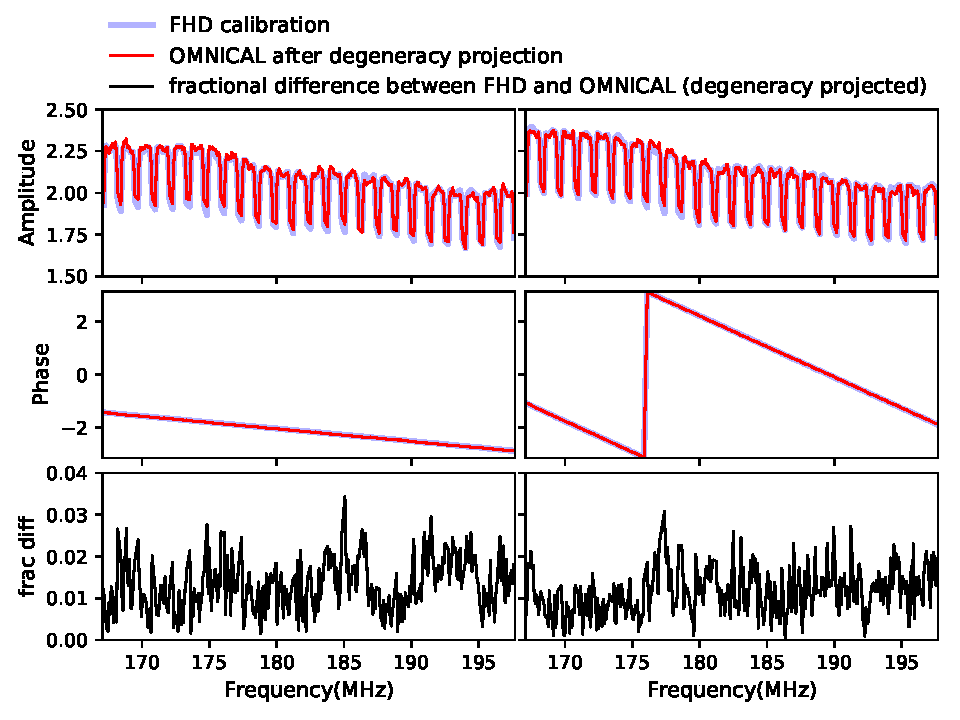
\includegraphics[width=0.85\linewidth]{figures/projtest2.pdf}}
\caption{30 minutes averaged gain calibrations of 2 MWA PhaseII tiles. Upper: Gain amplitude; Middle: Gain phase. Lower: fractional difference between sky based (FHD) and redundancy based (OMNICAL) solutions with degeneracy projected. Blue: FHD solutions; Red: OMNICAL solutions after projecting degeneracy.}
\end{figure}


%----------------------------------------------------------------------------------------
%	RESULTS 
%----------------------------------------------------------------------------------------

\section*{Murchison Widefield Array (MWA)}

The Murchison Widefield Array is one of the three Square Kilometer Array (SKA) Precursor telescopes located at the Murchison Radio-astronomy Observatory (MRO) in Western Australia, hunting for the intergalactic hydrogen gas during the Epoch of Reionization. It is a low frequency telescope operating at 80-300MHz, with a processed bandwidth of 30.72 MHz. The Phase I of MWA consists of 128 tiles pseudo-randomly distributed over 3 km diameter area. The newly upgraded Phase II of the MWA has the additional 128 tiles installed, with 72 of them forming into two hexagonal cores. 
\begin{figure}[H]
\centering
\label{fig:HERA}
\frame{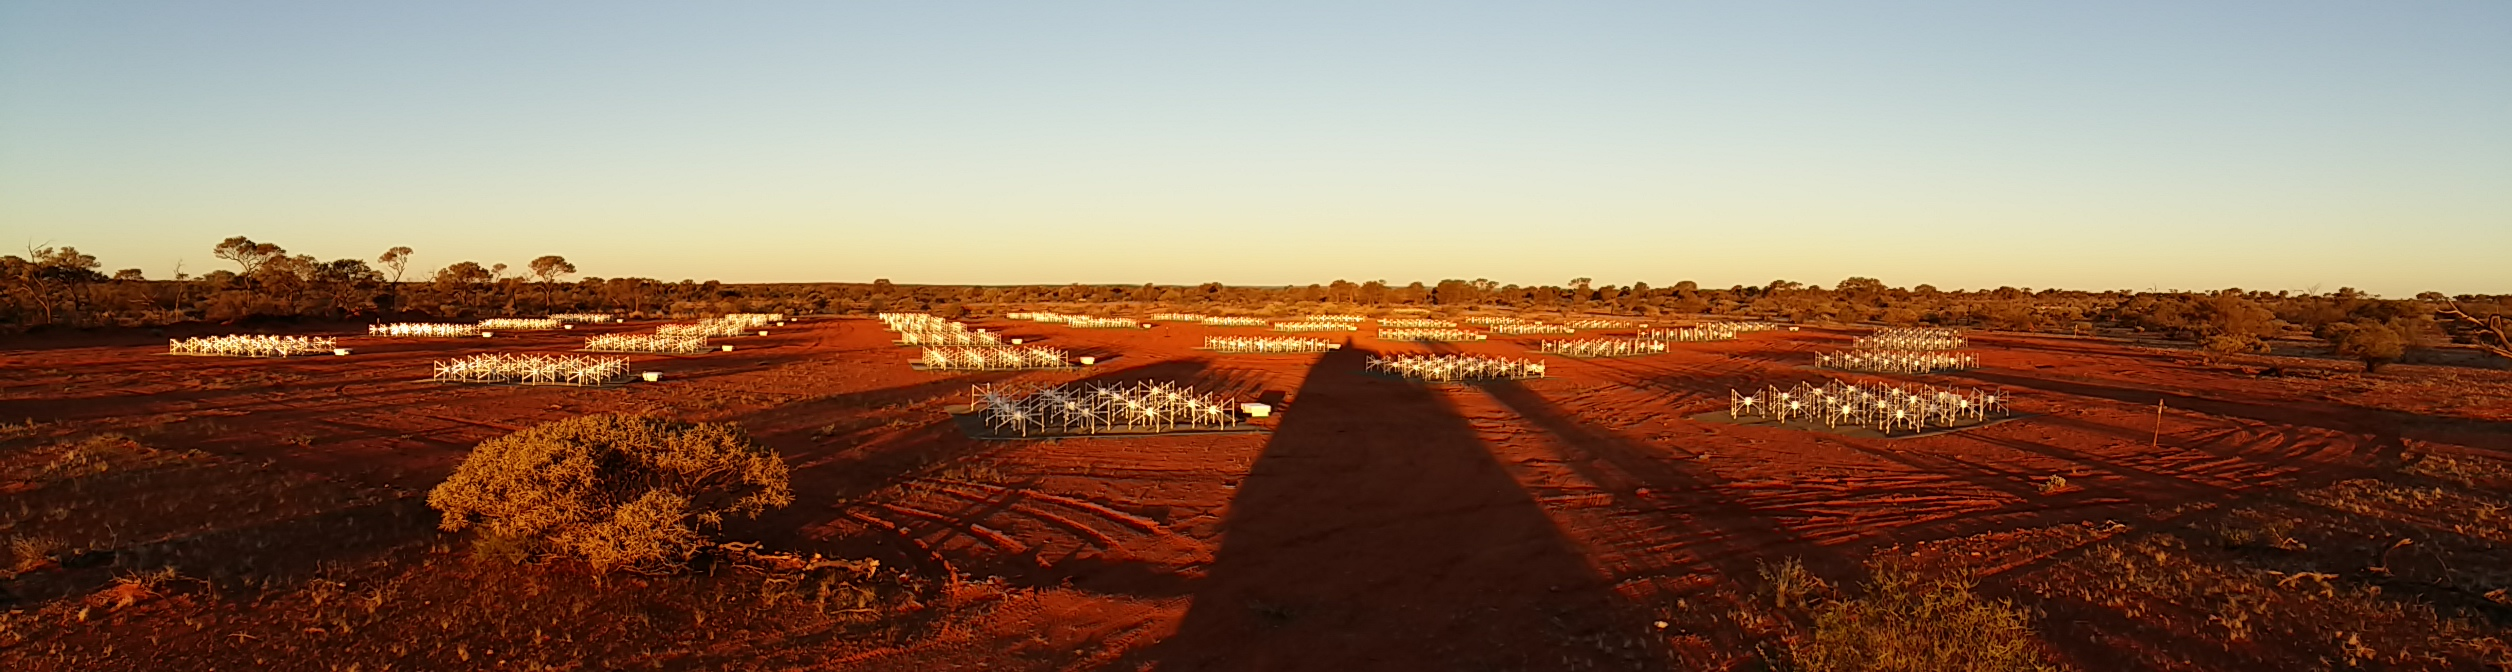
\includegraphics[width=0.95\linewidth]{figures/MWA_tiles.jpg}}
\caption{MWA - Located in the Murchison Radio-astronomy Observatory in Western Australia.}
\end{figure}


\section*{Hydrogen Epoch of Reionization Array (HERA)}
%\begin{figure}[H]
%\centering
%\label{fig:PAPER}
%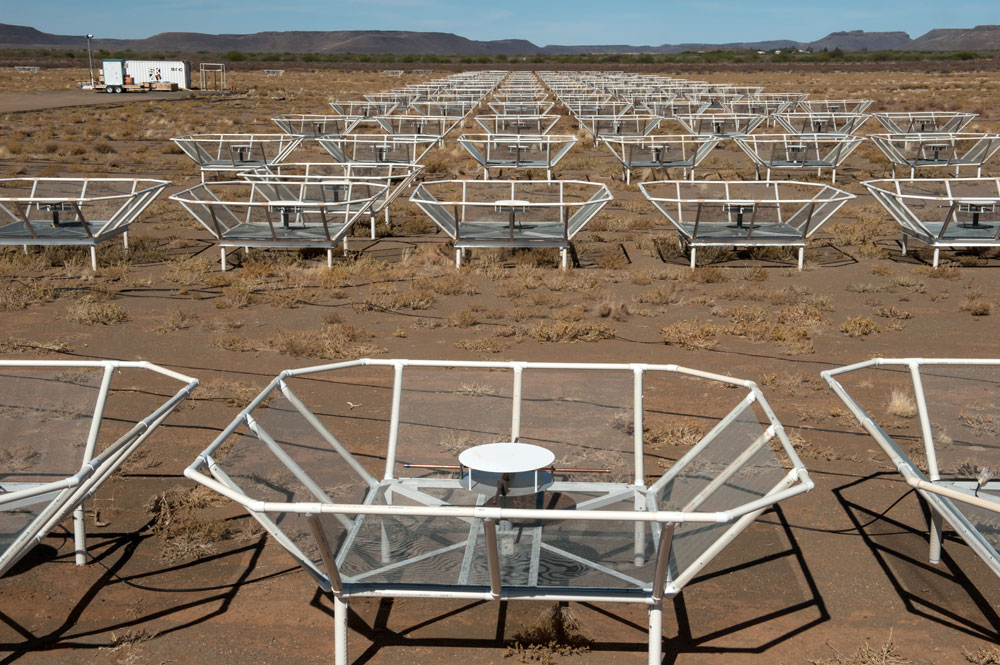
\includegraphics[width=0.85\linewidth]{figures/paper}
%\caption{PAPER - A first-generation array located in the Karoo desert of South Africa. Designed specifically for EoR research, PAPER is designed for maximum redundancy. Several baselines sample each $k_\perp$ modes, which allows for the use of redundant calibration.}
%\end{figure}

%\begin{figure}[H]
%\centering
%\label{fig:MWA}
%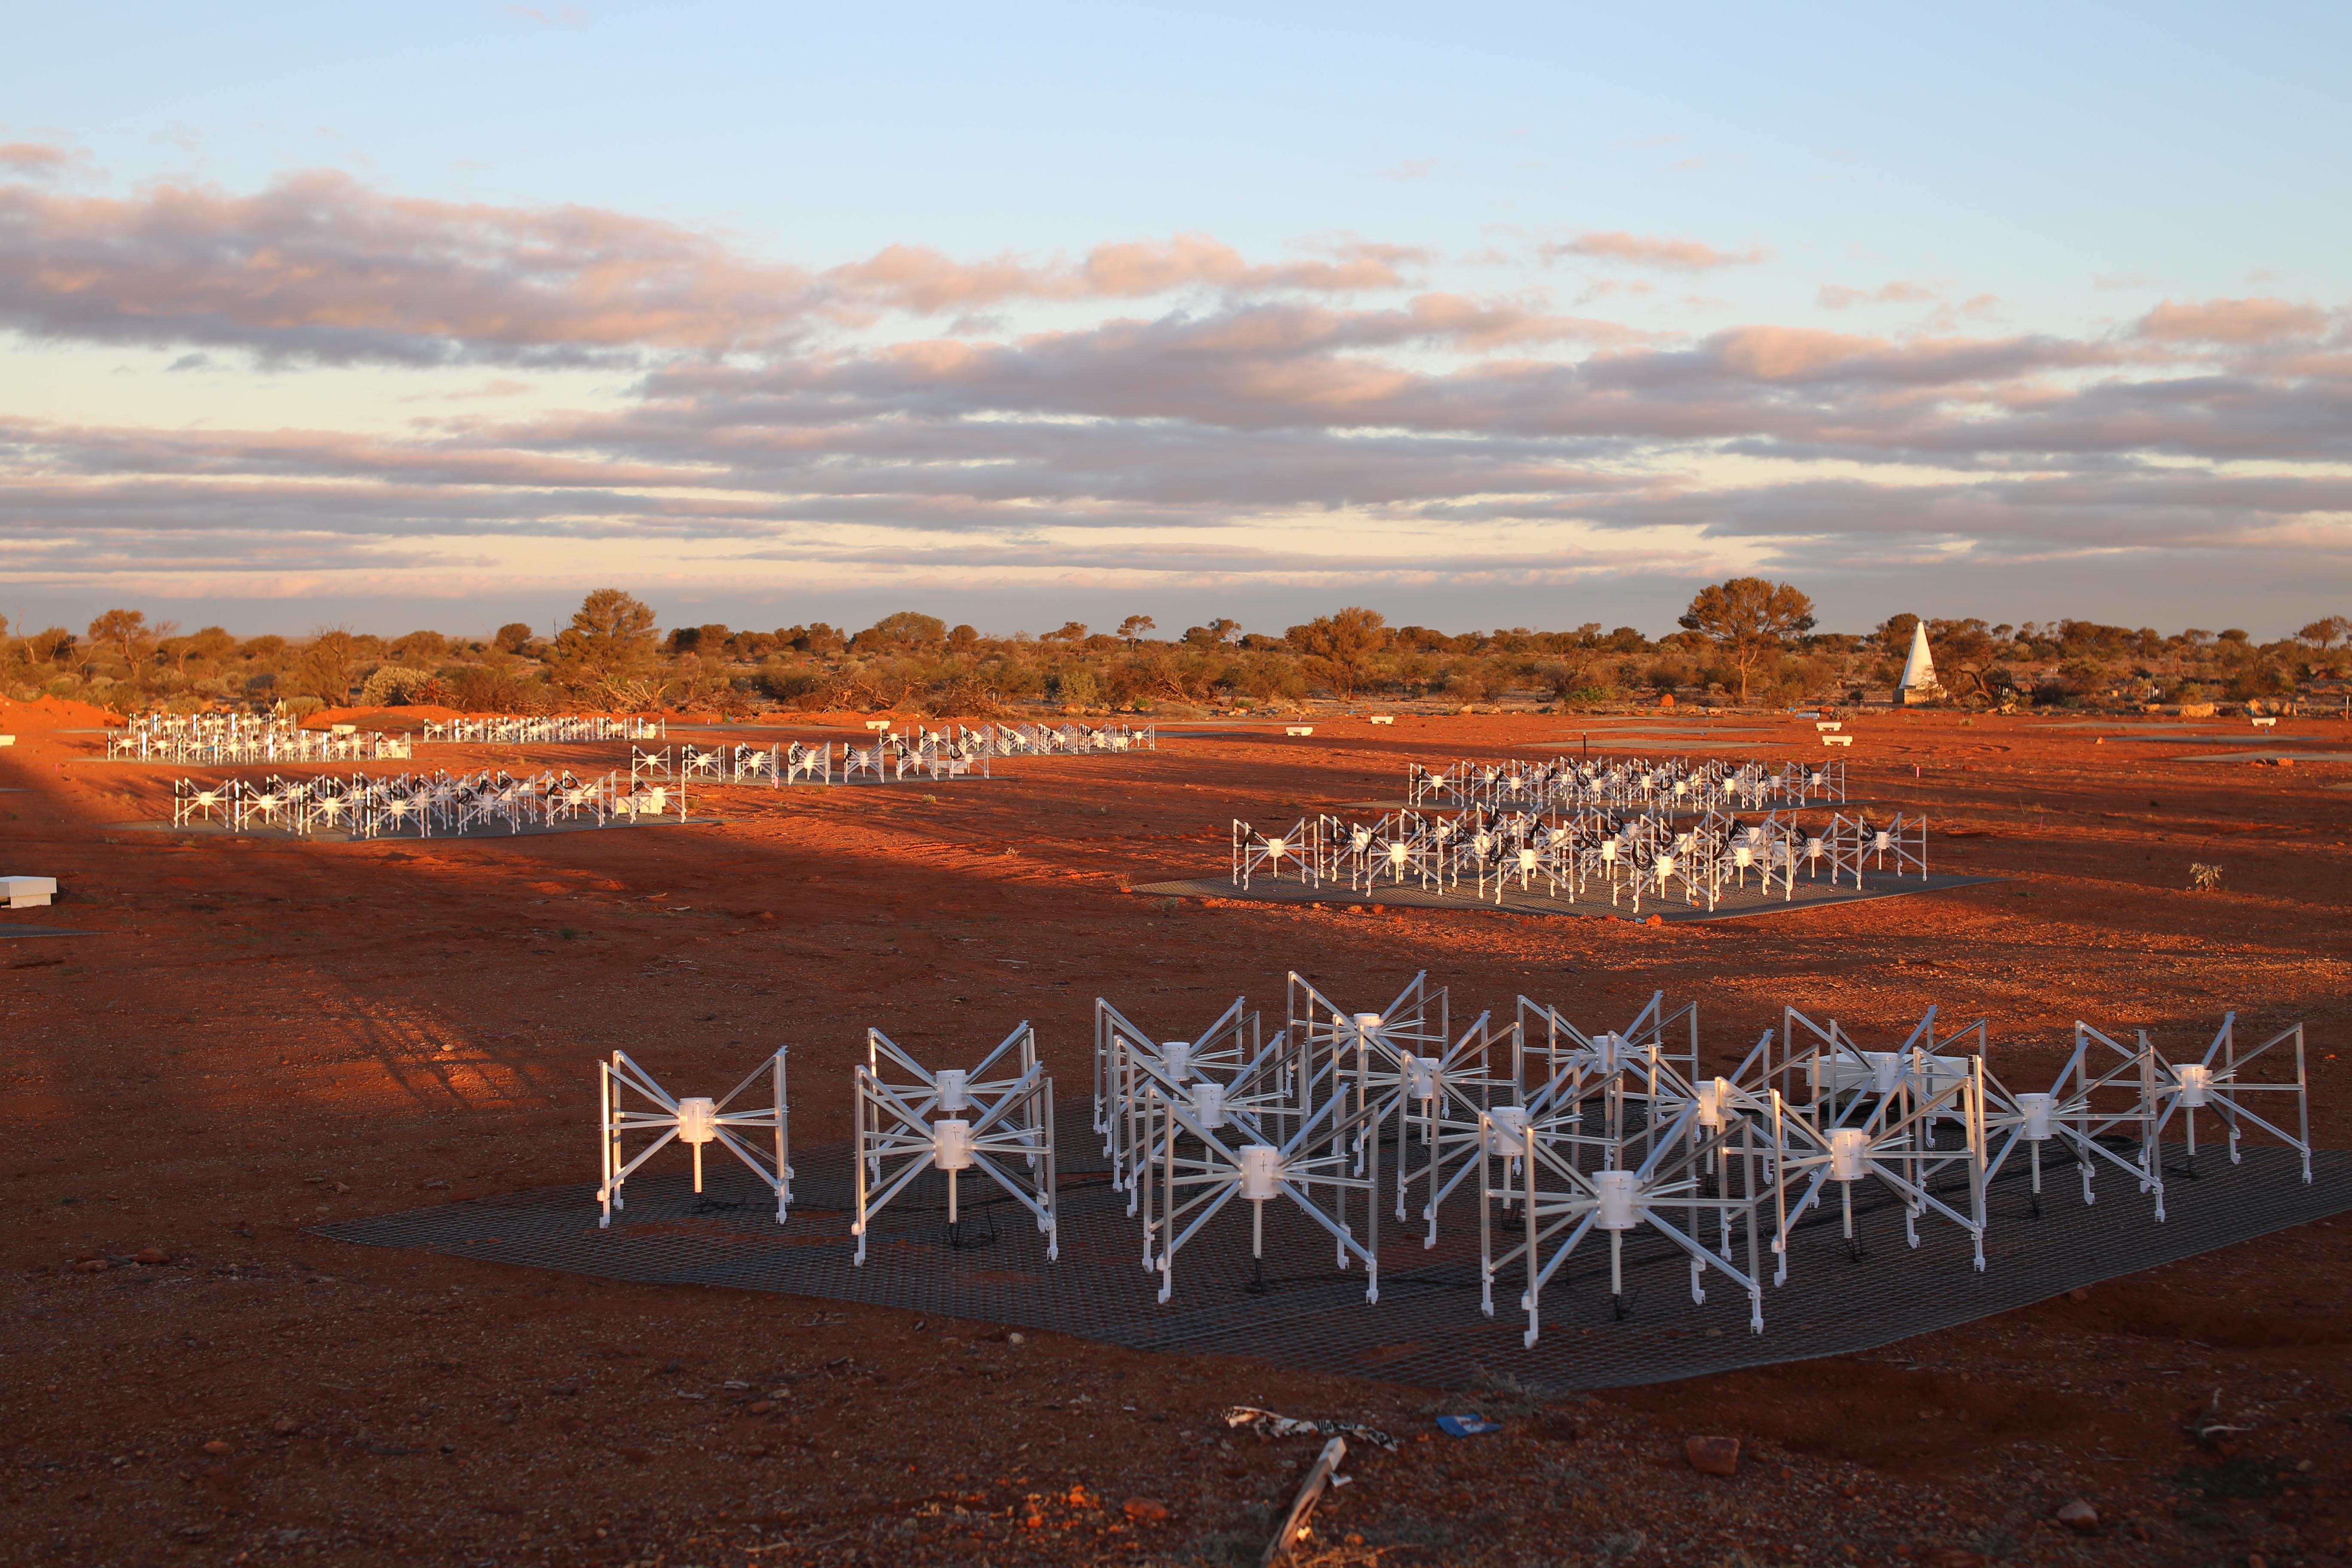
\includegraphics[width=0.85\linewidth]{figures/phaseII_tiles.jpg}
%\caption{MWA - Located in Western Australia at the Murchison Radio Astronomy Observatory. The MWA serves multiple functions, including ionosphere studies and detection of transient radio signals. Phase I consisted of 128 tiles which are each made up of 16 dipole antennae. The Phase I configuration maximized uv coverage, improving imaging capability. It has since been partially reconfigured into Phase II, which includes two hexagonal grids of tiles designed for high-redundancy EoR research. MWA is a pathfinder project for the Square Kilometer Array (SKA).}
%\end{figure}
The Hydrogen Epoch of Reionization Array is a $2^{nd}$ generation radio interferometer observing the 21 cm emission from neutral hydrogen during the Epoch of Reionization. HERA will eventually be an array with 350 14-meter parabolic dishes in South Africa. These elements will be divided into a 320-element hexagonal shaped core and 30 outriggers. The current stage of HERA has 37 dishes deployed and observing. 

%Although increasingly stringent upper limits of the 21 cm signal have been placed by the first generation experiments targeting the EoR such as the Precision Array for Probing the Epoch of Reionization array (PAPER), Murchison Widefield Array (MWA) and LOw Frequency ARray (LOFAR), they are not able to detect it due to their sensitivity limits (see Fig. \ref{fig:HERAsense}). HERA is designed to bring both the sensitivity and precision required to directly constrain the topology and evolution of reionization. By understanding the evolution of reionization we can better comprehend the formation of the first stars and earliest galaxies.\\

\begin{figure}[H]
\centering
\label{fig:HERA}
\frame{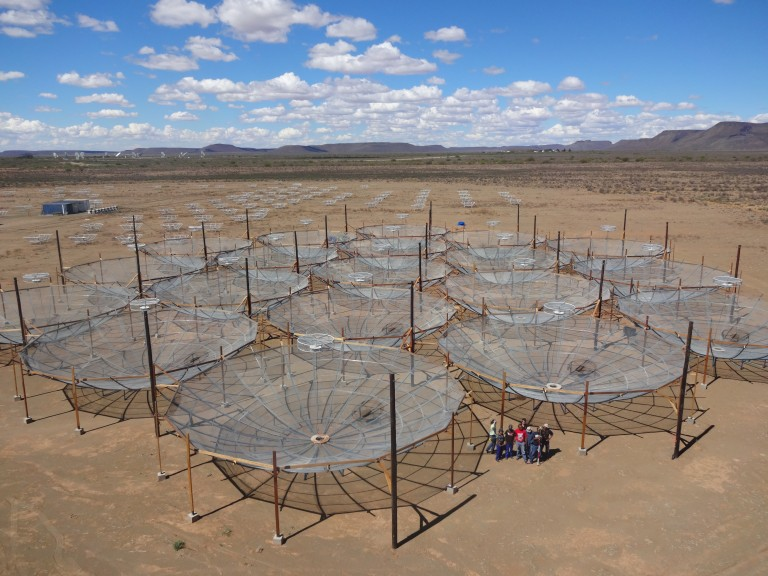
\includegraphics[width=0.85\linewidth]{figures/HERA19.png}}
\caption{HERA - Located in the Karoo desert in South Africa}
\end{figure}

%\begin{figure}[H]
%\centering
%\frame{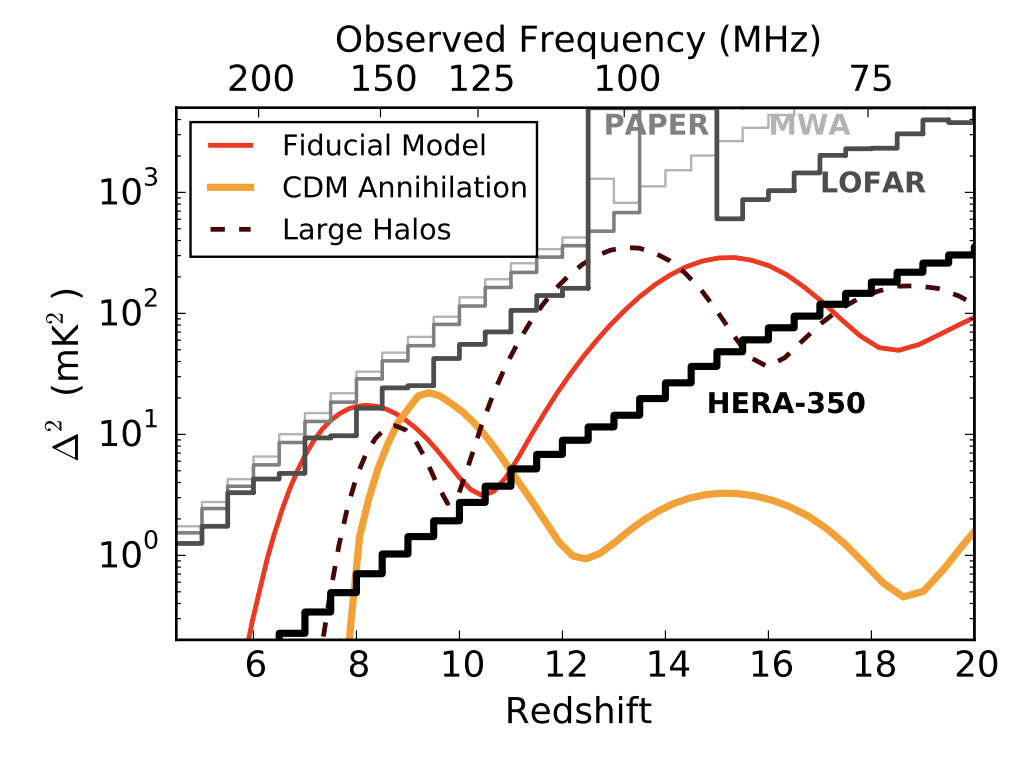
\includegraphics[width=0.9\linewidth]{figures/HERAsensitivity.png}}
%\caption{Projected SNR comparison of the 350 element phase of HERA (with 1080 hrs integration time) to other low frequency arrays. Relative to several reionization models (colored), HERA-350
%should have the sensitivity to measure the 21cm EoR signal across multiple redshifts. Source: DeBoer \& HERA Collaboration. PASP (2017).}
%\label{fig:HERAsense}
%\end{figure}

%----------------------------------------------------------------------------------------
%	CONCLUSIONS
%----------------------------------------------------------------------------------------

%\color{SaddleBrown} % SaddleBrown color for the conclusions to make them stand out

%\section*{Conclusions}

%[Do we have conclusions?] [No?]
\section*{}
\fbox{\begin{minipage}{0.95\linewidth}
\large \textbf{We are open to undergraduate and graduate students who are interested in our potential research projects. Feel free to contact us if you would like to join!}
\end{minipage}}

\color{DarkSlateGray} % Set the color back to DarkSlateGray for the rest of the content

%----------------------------------------------------------------------------------------
%	FORTHCOMING RESEARCH
%----------------------------------------------------------------------------------------

%\section*{Forthcoming Research}
%Probably not necessary because we can just add a blurb in the Radio Telescope arrays section about HERA?
%[Picture of HERA-331?]


 %----------------------------------------------------------------------------------------
%	REFERENCES
%----------------------------------------------------------------------------------------
% We referenced all the best people
%\nocite{*} % Print all references regardless of whether they were cited in the poster or not
%\bibliographystyle{plain} % Plain referencing style
%\bibliography{sample} % Use the example bibliography file sample.bib

%----------------------------------------------------------------------------------------
%	ACKNOWLEDGEMENTS
%----------------------------------------------------------------------------------------

%\section*{Acknowledgements}
%I refuse to acknowledge anyone or any thing!!!!!!!


%----------------------------------------------------------------------------------------
\end{multicols}
%\begin{minipage}[b]{0.19\linewidth}
%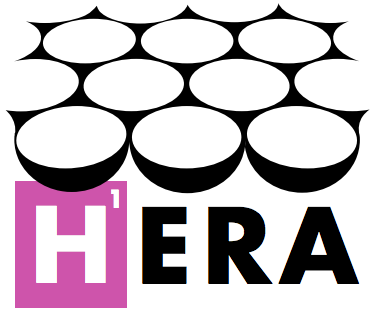
\includegraphics[width=15cm]{HERA.png} % Logo or a photo of you, adjust its dimensions here
%\end{minipage}
%\hspace{2cm}
%\begin{minipage}[b]{0.25\linewidth}
%\Huge{\textbf{PAPER}}
%\end{minipage}
%\hspace{2cm}
%\begin{minipage}[b]{0.25\linewidth}
%\Huge{\textbf{MWA}}
%\end{minipage}
\end{document}
